\chapter{Thermodynamics}
\section{Entropy and the Boltzmann law} 
\label{chapter1}
This section is adapted from Chatpers 2 and 5 of \cite{dill}. 
\begin{defi}[Equilibrium]
An equilibrium defines where a system tends to go and stay, \ie the net force \textit{analogue} on the system is zero. 
\end{defi}
\begin{defi}[Extremum principles]
An \textit{extremum principle} is a principle stating that a macrostate with most number of microstates are the most probable macrostate. 
\end{defi}
\begin{post}[Statistical definition of entropy]
\label{entropy}
The statistical definition of entropy, which follows from a \textit{principle of fair apportionment}, states that 
\begin{equation}
\label{eq:entr}
S=k\ln(W)
\end{equation}
\end{post}
We will be showing the intuitions behind \Cref{entropy} shortly, but we will first show that the alternative definition that 
\begin{equation}
\frac{S}{k}=-\sum^t_{i=1}p_i\ln(p_i)
\end{equation}
is equivalent to \Cref{eq:entr}: 
Roll a $t$-sided die $N$ times. The multiplicity of outsomes is given by 
\begin{equation}
W=\frac{N!}{n_1!n_2!\cdots n_t!}, 
\end{equation}
where $n_i$ is the number of times side $i$ appears face up. \\
\textit{Stirling's approximation} gives that 
\begin{equation}
x!\approx\left(\frac{x}{e}\right)^x, 
\end{equation}
and expressing probabilities $p_i=n_i/N$, we have
\begin{equation}
\begin{aligned}
W&=\frac{(N/e)^N}{(n_1/e)^{n_1}(n_2/e)^{n_2}\cdots (n_t/e)^{n_t}} \\
&=\frac{1}{p_1^{p_1}p_2^{p_2}\cdots p_t^{p_t}}\\
&\tf\ln(W)=-\sum^{t}_{i=1}n_i\ln{p_i} \\
&\imp\frac{1}{N}\ln{W}=-\sum^{t}_{i=1}p_i\ln{p_i}=\frac{S_N}{Nk}=\frac{S}{k}, 
\end{aligned}
\end{equation}
where $S_N$ is the total entropy for $N$ trials. 

The \textbf{central problem} of statistical thermodynamics is to infer the probability distribution from an observable quantity. 
\begin{thrm}[Flat distribution from no constraints]
The principle of maximising entropy leads to a flat probability distribution when there are no constraints. 
\end{thrm}
\begin{proof}
This is essentially a lagrange multiplier problem with
\begin{subequations}
\begin{align}
\text{objective function:\ }&S(p_1,p_2,...,p_t)=-k\sum_{i=0}^t p_i\ln{p_i} \\
\text{constraint function:\ }&\sum_{i=1}^{t}p_i=1\ \imp\sum^t_{i=1}\dif p_i=0
\end{align}
\end{subequations}
We hence construct the multiplier function  
\begin{equation}
L(p_i,\lambda)\equiv S-\lambda\left[\left(\sum_{i=1}^{t}p_i\right)-1\right]
\end{equation}
Maximising requires 
\begin{equation}
\nab L=0
\end{equation}
This implies 
\begin{equation}
-1-\ln(p_i)-\lambda=0\ \imp p_i^*=e^{-1-\lambda}, 
\end{equation}
where $*$ indicates maximised. 
We observe that this is a flat probability distribution (subject to normalisation). 
\end{proof}
\begin{thrm}[Boltzmann distribution]
However, if there is bias/constraint present, we can show that an exponential distribution results. 
\end{thrm}
\begin{proof}
The problem is now summarised as follows
\begin{enumerate}
\item A generalised die has $t$ sides, 
\item A 'score' $\epsilon_i$ is associated with the $i$-th side, 
\item The only observable quantity is 
	\begin{equation}
	\langle\epsilon\rangle\equiv\sum^t_{i=1}p_i\epsilon_i. 
	\end{equation}
\end{enumerate}
We seek to find the distribution of $p_i^*$. Again this is a lagrange multiplier problem with 
\begin{subequations}
\begin{align}
\text{objective function:\ }&S(p_1,p_2,...,p_t)=-k\sum_{i=0}^t p_i\ln{p_i} \\
\text{constraint function 1:\ }&g(p_i)\equiv\sum^t_{i=1}p_i=1 \label{lag_unity}\\
\text{constraint function 2:\ }&h(p_i)\equiv\sum^t_{i=1}p_i\epsilon_i=\langle\epsilon\rangle \label{lag_exp}
\end{align}
\end{subequations}
We again require that
\begin{equation}
\nab L\equiv\nab\left(S-\lambda g-\mu h\right)=0
\end{equation}
We have
\begin{subequations}
\begin{align}
&-1-\ln(p_i^*)-\lambda-\mu\epsilon_i=0 \\
&p^*_i=e^{-1-\lambda-\mu\epsilon_i} \\
&p_i^*=\frac{p_i^*}{\sum_{i=1}^t p_i^*}=\frac{e^{-\mu\epsilon_i}}{\sum_{i=1}^t e^{-\mu\epsilon_i}}\label{boltzmann}, 
\end{align}
\end{subequations}
We can express $\langle\epsilon\rangle$ in terms of the distribution from \Cref{lag_exp}: 
\begin{equation}
\label{boltz_exp}
\langle\epsilon\rangle=\sum^t_{i=1}\epsilon_ip^*_i=\frac{1}{q}\sum^t_{i=1}\epsilon_ie^{-\mu\epsilon_i}. 
\end{equation}
\end{proof}

\begin{defi}[Boltzmann distribution law and partition function]
\Cref{boltzmann} is known as the \textbf{Boltzmann distribution law}, and the quantitiy in the denominator is known as the \textbf{partition function} $q$. 
\end{defi}

\begin{wex}[Bias in dice]
Suppose we have a $6$-faced die and the score on each face is the index, \ie $\epsilon_i=i$. \\
The Boltzmann distribution law of \Cref{boltzmann} gives
\begin{equation}
\label{ex_die1}
p^*_i=\frac{e^{-\mu i}}{\sum^6_{i=1}e^{-\mu i}}. 
\end{equation}
And from \Cref{boltz_exp} we have
\begin{equation}
\begin{aligned}
\label{ex_die2}
\langle\epsilon\rangle&=\sum^6_{i=1}ip^*_i \\
&=\frac{e^{-\mu}+2e^{-2\mu}+3e^{-3\mu}+4e^{-4\mu}+5e^{-5\mu}+6e^{-6\mu}}{e^{-\mu}+e^{-2\mu}+e^{-3\mu}+e^{-4\mu}+e^{-5\mu}+e^{-6\mu}}. 
\end{aligned}
\end{equation}
\Cref{ex_die2} is an equation with one unknown, $\mu$. 
Simple algebra can show that if $\langle\epsilon\rangle=3.5$, $\mu=0$ and a flat distribution is resulted, 
and if $\langle\epsilon\rangle<3.5$, $\mu<0$ and \textit{vice versa}. 
\end{wex}

\section{The fundamental thermodynamic equations}
This section is adapted from \cite{dill} unless otherwise stated. 
\begin{thrm}[Fundamental equations]
The \textbf{fundamental thermodynamic equations for entropy and energy} are 
\begin{subequations}
\begin{align}
S&=S(U,V,\boldsymbol{N}) \\
U&=U(S,V,\boldsymbol{N})
\end{align}
\end{subequations}
respectively, where $\boldsymbol{N}$ means $N_1,N_2,\dots,N_M$. These equations \textit{predict equilibria}. 
\end{thrm}
Both equations can completely specify the state of a simple system. 
These equations does \textit{not} tell you the mathematical dependences, instead, 
\textit{equations of state}, such as the ideal gas law, specify the interrelations 
among these variables. 
These must come from experiments or microscopic models. 
\subsection{The fundamental equations}
Taking the total differential of $S$ and $U$ we have
\begin{subequations}
\begin{align}
\dif S&=\diffp SU[V,\boldsymbol{N}]\dif U+\diffp SV[U,\boldsymbol{N}]\dif V+\sum_{j=1}^M\diffp {S}{N_j}[U,V,N_{i\neq j}]\dif N_j \label{fund_a}\\
\dif U&=\diffp US[V,\boldsymbol{N}]\dif S+\diffp UV[S,\boldsymbol{N}]\dif V+\sum_{j=1}^M\diffp {U}{N_j}[S,V,N_{i\neq j}]\dif N_j \label{fund_b}
\end{align}
\end{subequations}
From these expressions we make the following definitions: 
\begin{defi}[Basic thermodynamic quantities]
\begin{subequations}
\begin{align}
\text{the temperature:\ }&T=\diffp US[V,\boldsymbol{N}] \label{diff_t}\\
\text{the pressure:\ }&p=-\diffp UV[S,\boldsymbol{N}] \label{diff_p}\\
\text{the chemical potential:\ }&\mu_j=\diffp {U}{N_j}[S,V,N_{i\neq j}]\label{diff_mu}
\end{align}
\end{subequations}
We now have, by way of definition, 
\begin{subequations}
\begin{align}
\dif U&=T\dif S-p\dif V+\sum_{j=1}^M\mu_j\dif N_j \label{diff_a}\\
\dif S&=\left(\frac{1}{T}\right)\dif U+\left(\frac{p}{T}\right)\dif V-\sum_{j=1}^M\left(\frac{\mu_j}{T}\right)\dif N_j \label{diff_b}, 
\end{align}
\end{subequations}
where \Cref{diff_b} is obtained by algebraic rearrangement of \Cref{diff_a} and gives us three further definitions: 
\begin{subequations}
\begin{align}
\frac{1}{T}&=\diffp SU[V,\boldsymbol{N}] \label{sdiffa}\\
\frac{p}{T}&=\diffp SV[U,\boldsymbol{N}] \label{sdiffb}\\
\frac{\mu_j}{T}&=\diffp{S}{N_j}[U,V,N_{i\neq j}]. \label{sdiffc}
\end{align}
\end{subequations}
\end{defi}
We will show that \Cref{diff_a,diff_b} can be used to identify states of equilibrium shortly. In the following section we first show the derivation of the ideal gas law. 

\subsection{The ideal gas law}
\begin{thrm}[The ideal gas law]
The ideal gas law is stated as
\begin{equation}
\label{idealgl}
pV=NkT. 
\end{equation}
\end{thrm}
\begin{proof}
Imagine a lattice of $M$ sites for $N$ particles where $M\geq N$, the multiplicity $W$ is computed by 
\begin{equation}
W=\frac{M!}{N!(M-N)!}. 
\end{equation}
Hence the entropy is 
\begin{equation}
S=k\ln(W(N,M))=\ln\left[\frac{M!}{N!(M-N)!}\right].
\end{equation}
We now in effect knows how the entropy depends on volume, and that's handy because 
\Cref{sdiffb} gives us a way to get an expression for $p$. \\
In our model, we assert that $V/M=v_0$, the volume per lattice site, which is a constant. 
We can now write 
\begin{equation}
\diffp SV[N]=\diff SM[N]\left(\diff MV \right)=\diffp SM[N]\left(\frac{1}{v_0}\right). 
\end{equation}
We still have $\diffp S/M[N]$ to calculate: 
\begin{subequations}
\begin{align}
\frac{S}{k}&=\ln(W(N,M))=\ln\left[\frac{M!}{N!(M-N)!}\right]\\
&=M\ln M-N\ln N-(M-N)\ln(M-N) \\
&=-N\ln\left(\frac{N}{M}\right)-(M-N)\ln\left(\frac{M-N}{M}\right) \\
\imp\diffp SM[N]&=k\left[1+\ln M-\ln(M-N)-\frac{M-N}{M-N}\right] \label{igl4}\\
&=-k\ln\left(1-\frac{N}{M}\right), \label{igl5}
\end{align}
\end{subequations}
where \Cref{igl4} results from rewriting $(M\ln M)$ into $(N\ln M) + [(M-N)\ln M]$. \\
We perform a Taylor series expansion on \Cref{igl5}, in the limit that $N/M\ll1$: 
\begin{subequations}
\begin{align}
p&=\frac{T}{v_0}\diffp SM[N] \\
&=-kT\left(\frac{M}{V}\right)\ln\left(1-\frac{N}{M}\right) \\
&\approx\left(-\frac{MkT}{V}\right)\left(-\frac{N}{M}\right)\left[1+\frac{1}{2}\left(\frac{N}{M}\right)+\cdots\right] \\
&\approx\frac{NkT}{V}, 
\end{align}
\end{subequations}
which yields the ideal gas law. Higher-order terms give further refinements, such as the \textit{van der Waals equation}, which includes the first-order correction. 
\end{proof}
\begin{coro}[Entropy of ideal gas]
As given by \Cref{sdiffb,idealgl}, we can write, for an ideal gas, 
\begin{subequations}
\begin{align}
\diffp SV[U,\bvec{N}]&=\frac{Nk}{V} \\
S(V,\bvec{N})&=Nk\ln V. 
\end{align}
\end{subequations}
\end{coro}

\subsection{Second law and equilibria}
\begin{defi}[Extensive and intensive quantities]
\textit{Extensive quantities} are additive and depend on the size of the system, such as internal energy, entropy, volume and number of particles. \\
\textit{Intensive quantities} are not additive and do not depend on the size of the system, such as temperature and pressure. 
\end{defi}
\begin{defi}[First-order homogeneous function]
Since $U=U(S,V,\bvec{N})$ is a function of all extensive quantities, $U$ itself is an extensive quantity as well. Furthermore, $U$ has the important property of being a \textit{first-order homogeneous function}, which behaves as 
\begin{equation}
f(\lambda x)=\lambda f(x).
\end{equation}
This leads to the important property: 
\end{defi}
\begin{prt}[Derivative of first-order homogeneous functions]
Because, for a first-order homogeneous function, 
\begin{equation}
\diff{f(\lambda x)}{(\lambda x)}=\diff{[\lambda f(x)]}{x}\diff{x}{(\lambda x)}=\diff{f}{x}, 
\end{equation}
\ie its derivative with respect to an extensive variable is an \textit{intensive variable}. 
\end{prt}
Therefore, we can conclude from \Cref{diff_t,diff_p,diff_mu} that $T$, $p$ and $\mu$ are intensive quatities and do not depend on systme size.
\subsubsection{The second law}
\begin{post}[The second law]
The second law states that isolated systems tend toward their states of maximum entropy. 
\end{post}
We will show that this predicts states of equilibrium. 
\begin{thrm}[Thermodynamic forces]
It can be shown that $1/T$ is a measure of a systyem's tendency for heat exchange, 
$p/T$ is a measure of a system's tendency for volumn exchange, 
and $\mu/T$, particle exchange.
\end{thrm}
The strategy to do so is to
\begin{enumerate}
\item Determine the relevant independent variables, 
\item Apply the fundamental entropy equation and the constraints, 
\item Use the maximum entropy principle, \ie the second law to specify the state of equilibrium. 
\end{enumerate}
\begin{proof}[Temperature]
We need to demonstrate that temperature as defined by \Cref{diff_t} satisfies the notion of temperature given as: 
\begin{itemize}
	\item It is the quantity that tells you when heat exchange will occur, and
	\item objects exchange heat to reach a state of maximum entropy, and
	\item in this state their temperatures are equal. 
\end{itemize}
Imagine two objects $A$ and $B$ are brought into thermal contact. 
They can only exchange energy with each other not the surroundings, 
and no particle or volume exchange is possible either. 
We are interested to know how the entropy of the objects depend on the energy: $S_A(U_A)$ nad $S_B(U_B)$. \\
Say object $A$ has energy $U_A$, entropy $S_A$ and $1/T_A=(\diffp{S_A}/{U_A})$ and likewise for $B$. \\
Entropy is an extensive property, so
\begin{equation}
\label{stotal}
S_{total}=S_A+S_B. 
\end{equation}
\Cref{stotal} does not mean that $S_{total}$ is fixed however. We obtain an equation likewise for total internal energy
\begin{equation}
\label{utotal}
U_{total}=U_A+U_B=\text{constant},  
\end{equation}
which is the constraint equation. 
To find the state of thermal equilibrium, we apply the second law, \ie
\begin{equation}
\dif S=0.
\end{equation}
We therefore have, for $\dif V=\dif\bvec{N}=0$, 
\begin{equation}
\label{diff_s}
\dif S_{total}=\dif S_A+\dif S_B=\diffp{S_A}{U_A}[V,\bvec{N}]\dif U_B+\diffp{S_B}{U_B}[V,\bvec{N}]\dif U_B=0. 
\end{equation}
The differential form of the constraint equation \Cref{utotal} is 
\begin{equation}
\label{diff_constr}
\begin{aligned}
&\dif U_A+\dif U_B=\dif U_{total}=0 \\
\imp&\dif U_A=-\dif U_B
\end{aligned}
\end{equation}
Substitute \Cref{diff_constr} into \Cref{diff_s} and rearrage to get 
\begin{subequations}
\begin{align}
\dif S_{total}&=\left[\diffp{S_A}{U_A}[V,\bvec{N}]-\diffp{S_B}{U_B}[V,\bvec{N}]\right]\dif U_A=0 \\
&\imp\diffp{S_A}{U_A}[V,\bvec{N}]=\diffp{S_B}{U_B}[V,\bvec{N}]\\
&\imp\frac{1}{T_A}=\frac{1}{T_B}\imp T_A=T_B. 
\end{align}
\end{subequations}
\end{proof}
\begin{proof}[Pressure]
Consider a cylinder partitioned into subsystems $A$ and $B$, with only volume exchange possible. This also means that $T_A=T_B$ since no energy exchange is possible. The constant volume and internal energy constraints leads to
\begin{subequations}
\label{constr_p}
\begin{align}
\dif V_A&=\dif V_B \\
\dif U_A&=\dif U_B. 
\end{align}
\end{subequations}
The second law gives
\begin{equation}
\dif S=\left(\diffp{S_A}{V_A}\right)\dif V_A+\left(\diffp{S_B}{V_B}\right)\dif V_B+\left(\diffp{S_A}{U_A}\right)\dif U_A+\left(\diffp{S_B}{U_B}\right)\dif U_B=0
\end{equation}
Applying contraints in \Cref{constr_p} gives 
\begin{equation}
\dif S=\left(\frac{p_A}{T_A}-\frac{p_B}{T_B}\right)\dif V_A + \left(\frac{1}{T_A}-\frac{1}{T_B}\right)\dif U_A=0, 
\end{equation}
Because $T_A=T_B$, we get, at equilibrium, 
\begin{equation}
p_A=p_B.
\end{equation}
\end{proof}
\begin{proof}[A statistical mechanical proof of pressure]
Consider a container of $M$ sites with $M_A$ and $M_B$ sites in the two sides. 
$N_A$ and $N_B$ are fixed. We want to find $M_A^*$ and $M_B^*$ that maximises the multiplicity function: 
\begin{equation}
\label{pres_mult}
W(N,M)=\frac{M!}{(M-N)!}\frac{1}{N!}. 
\end{equation}
For $N/M\ll1$, the approximation
\begin{equation}
\frac{M!}{(M-N)!}\approx M^N
\end{equation}
holds (nb. this is a rather trivial result of the limit and \textit{not} Stirling's approximation). Setting $M_B=M-M_A$, \Cref{pres_mult} can be reduced to 
\begin{equation}
\label{pres_simp}
W_{tot}=W_AW_B=\frac{M_A^{N_A}(M-M_A)^{N_B}}{N_A!N_B!}
\end{equation}
We are interested to know maximise $W$ in the form of the function $S=k\ln(W)$ with respect to the $M$'s: 
\begin{equation}
\diff{\ln W}{M_A}=0. 
\end{equation}
\Cref{pres_simp} gives us
\begin{equation}
\ln W=N_A\ln M_A+N_B\ln(M-M_A), 
\end{equation}
and taking logarithm we get 
\begin{equation}
\frac{N_B}{M_B^*}=\frac{N_A}{M_A^*}, 
\end{equation}
which is the desired result that equilibrium is reached when densities are equalised at low pressures.
\end{proof}
\begin{proof}[Chemical potential]
This proof is adapted from \cite{callen} as the argument given in \cite{dill} contains omissions. \\
Consider $N$ identical particles, divided into $N_A$ and $N_B$. Particle and energy exchange is allowed, but not volume. We thus have constraints
\begin{subequations}
\begin{align}
\dif N_A+\dif N_B&=0 \\
\dif U_A+\dif U_B&=0.
\end{align}
\end{subequations}
The second law requires
\begin{equation}
\dif S=\left(\frac{1}{T_A}-\frac{1}{T_B}\dif U_A \right)-\left(\frac{\mu_A}{T_A}-\frac{\mu_B}{T_B} \right)\dif N_A=0
\end{equation}
We have the conditions of equilibrium
\begin{subequations}
\begin{align}
\frac{1}{T_A}&=\frac{1}{T_B}\\
\frac{\mu_A}{T_A}&=\frac{\mu_B}{T_B}.
\end{align}
\end{subequations}
The conditions can be simplified if $T_A=T_B=T$, to
\begin{equation}
\dif S=\frac{\mu_B-\mu_A}{T}\dif N_A. 
\end{equation}
And since $\dif S\geq0$, we conclude that if $\mu_B<\mu_A$, $\dif N_A$ must be negative and hence matter flows from $A$ to $B$.
\end{proof}

\section{The first and second laws in depth}
This section is adapted from Chapters 11 through 14 of \cite{bl}. 
\subsection{The First Law}
\subsubsection{Energy}
The first law is essentially a statement of conservation of energy.
\begin{defi}[First Law]
Energy is conserved and heat and work are both forms of energy.
\end{defi}
Consevation of energy reasons that
\begin{equation}
\label{L1diff}
\dif U=\indiff Q+\indiff W.
\end{equation}
Only in a reversible process, \ie no turbulence, can we assert that
\begin{equation}
\label{workdiff}
\indiff W=-p\dif V
\end{equation}
\begin{defi}[Reversible Process]
	A \text{reversible process} is a process whose direction can be changed by an infinitesimal change in a system parameter. 
	These processes are called \textbf{quasistatic}.
\end{defi}
It turns out that physically internal energy $U$ is a function of temperature $T$ and volume $V$, \ie $U\equiv U(T,V)$. 
Therefore, 
\begin{equation}
\dif U=\diffp UT[V] \dif T + \diffp UV[T]\dif V
\end{equation}
Rearranging \Cref{L1diff} with \Cref{workdiff} we obtain, for \textit{reversible} processes
\begin{equation}
\label{heatcap}
\begin{split}
\indiff Q&=\diffp UT[V]\dif T+\left[\diffp UV[T]+p\right] \dif V \\
\frac{\indiff Q}{\dif T}&=\diffp UT[V] +\left[\diffp UV[T]+p\right]\diff VT
\end{split}
\end{equation}
\begin{defi}[Heat capacities]
\label{def:heatcap}
\begin{subequations}
\begin{align}
C_V&=\diffp QT[V] \\
C_p&=\diffp QT[p]
\end{align}
\end{subequations}
\end{defi}

From \Cref{heatcap} and \Cref{def:heatcap}, we identify
\begin{thrm}[Heat Capacities]
\begin{subequations}
\begin{align}
C_V&=\diffp UT[V] \label{eq:cv}\\
C_p&=\diffp UT[V]+\left[\diffp UV[T]+p\right]\diffp VT[p]. \label{eq:cp}
\end{align}
\end{subequations}
\end{thrm}

\begin{coro}[Monatomic Heat Capacities]
For an ideal monatomic gas, $U$ is given by $U=\frac{3}{2}RT$ per mole. Hence, 
\begin{equation}
\diffp UV[T]=0
\end{equation}
and according to the ideal gas law $V=\frac{RT}{P}$,
\begin{equation}
\diffp VT[p]=\frac{R}{p}.
\end{equation}
Therefore we have, from \Cref{eq:cv,eq:cp},
\begin{subequations}
\begin{align}
C_{V, m}&=\frac{3}{2}R \\
C_{p, m}&=\frac{5}{2}R.
\end{align}
\end{subequations}
\end{coro}

\begin{defi}[Adiabatic Index]
\label{defi:ad_ind}
\begin{equation}
\gamma \equiv \frac{C_p}{C_V}
\end{equation}
For a monatomic gas, 
\begin{equation}
\label{monat_ad}
\gamma = \frac{C_p}{C_V} = \frac{C_V+R}{C_V}=1+\frac{R}{C_V}=\frac{5}{3}.
\end{equation}
\end{defi}

\begin{coro}[U per unit mass and volume for Ideal Gases]
The internal energy of an ideal gas is given by $U=C_vT$, 
using $pV=Nk_BT$ and $\rho=Nm/V$, we get
\begin{equation}
\frac{p}{\rho}=\frac{k_BT}{m},
\end{equation} 
and from \Cref{monat_ad}, $C_V=\frac{R}{\gamma - 1}$, gives 
\begin{equation}
U=C_VT=\frac{RT}{\gamma - 1}=\frac{N_Ak_BT}{\gamma-1}.
\end{equation}
As molar mass is $mN_A$, dividing through by molar mass gives
\begin{equation}
\tilde{u}=\frac{p}{\rho\left(\gamma-1\right)},
\end{equation}
the internal energy per unit mass. 
It follows that the internal energy per unit volume is then simply
\begin{equation}
u=\rho\tilde{u}=\frac{p}{\gamma-1}
\end{equation}
\end{coro} 
As this is a reversible change, since we have $\Delta S=\Delta Q/T$, we can write the molar entropy change
\begin{equation}
	\Delta S=R\ln\frac{V_f}{V_i}.
\end{equation}

\subsubsection{Isothermal and Adiabatic Processes}
\begin{thrm}[Isothermal expansion heat]
In an isothermal process $\dif T\equiv0$, hence $\dif U=0$. 
This implies
\begin{equation}
\indiff W=-\indiff Q.
\end{equation}
\begin{equation}
\begin{aligned}
\Delta Q&=\int \indiff Q \\
&=\int \indiff W \\
&=\int_{V_1}^{V_2}p\dif V \\
&=\int_{V_1}^{V_2}\frac{RT}{V}\dif V \\
&=RT\ln\frac{V_2}{V_1}
\end{aligned}
\end{equation}
\end{thrm}

\begin{defi}[Adiabatic changes]
A change is \textbf{adiabatic} if it is both \textbf{thermally isolated} and \textbf{reversible}. 
This is also called an \textbf{isentropic} process. 
\end{defi}
\begin{lemma}[Properties of adiabatic changes]
\begin{subequations}
\begin{align}
\indiff Q&=0 \\
\dif U&=\indiff W
\end{align}
\end{subequations}
For an \textbf{ideal gas}, therefore 
\begin{subequations}
\begin{align}
C_V\dif T&=-p\dif V=-\frac{RT}{V}\dif V \\
\ln\frac{T_2}{T_1}&=-\frac{R}{C_V}\ln\frac{V_2}{V_1}. \label{eq:adia}
\end{align}
\end{subequations}
\Cref{defi:ad_ind} gives
\begin{equation}
\gamma=\frac{C_p}{C_V}=1+\frac{R}{C_V},
\end{equation}
\end{lemma}
Rearranging with \Cref{eq:adia} we arrive at 
\begin{thrm}[Adiabatic equation]
\begin{equation}
\begin{aligned}
TV^{\gamma-1}&=\text{constant}, \\
pV^{\gamma}&=\text{constant}, \\
T\left(\frac{T}{V}\right)^{\gamma-1}&=\text{constant}, \\
p^{1-\gamma}T^{\gamma}&=\text{constant}.
\end{aligned}
\end{equation}
\end{thrm}

\subsection{The Second Law}
\subsubsection{Heat Engines}
The second law concerns itself with the \textbf{direction} of heat flow as the system approaches equilibrium. 
\begin{defi}[The Second Law]
\label{L2}
A statement of the second law is that no process is possible whose sole result is the transfer of heat from a colder to a hotter body. 
\textbf{\textit{OR}} that no process is possible whose sole reulst is the complete conversion of heat into work. 
\end{defi}
\begin{figure}[!htbp]
	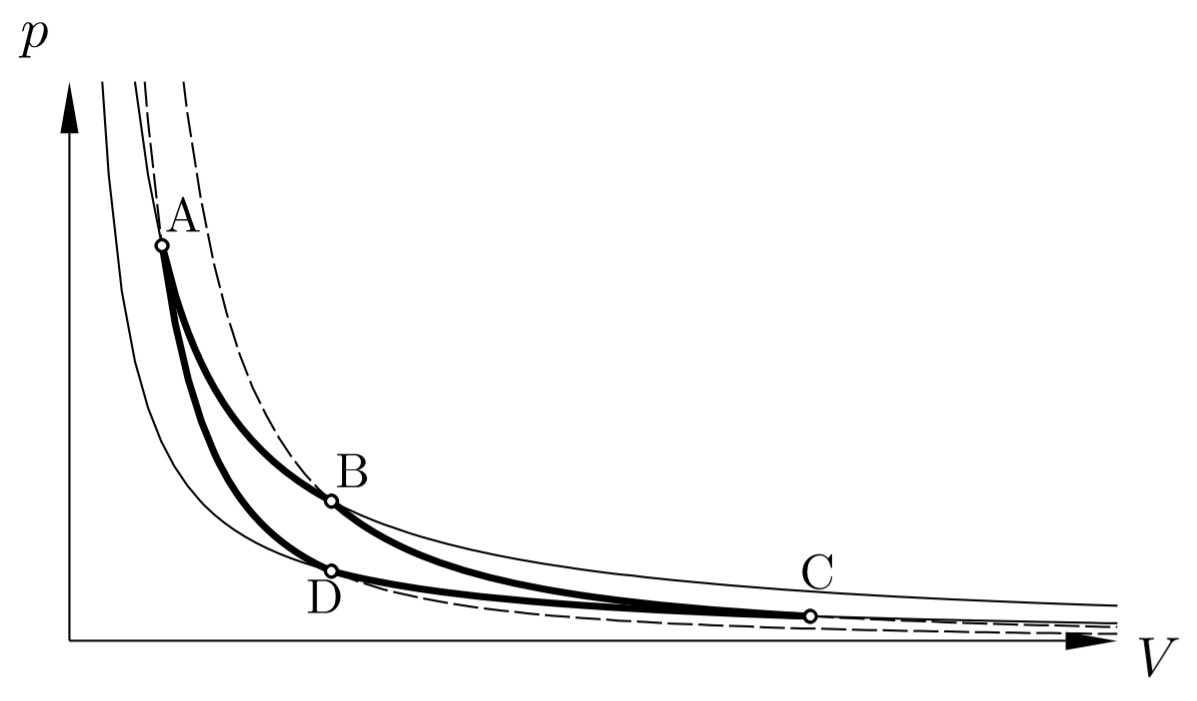
\includegraphics[width=8cm]{adia_pv}
	\centering
	\caption{A p-V plot of the Carnot cycle.}
	\label{fig:adia_pv}
\end{figure}
\begin{figure}[!htbp]
	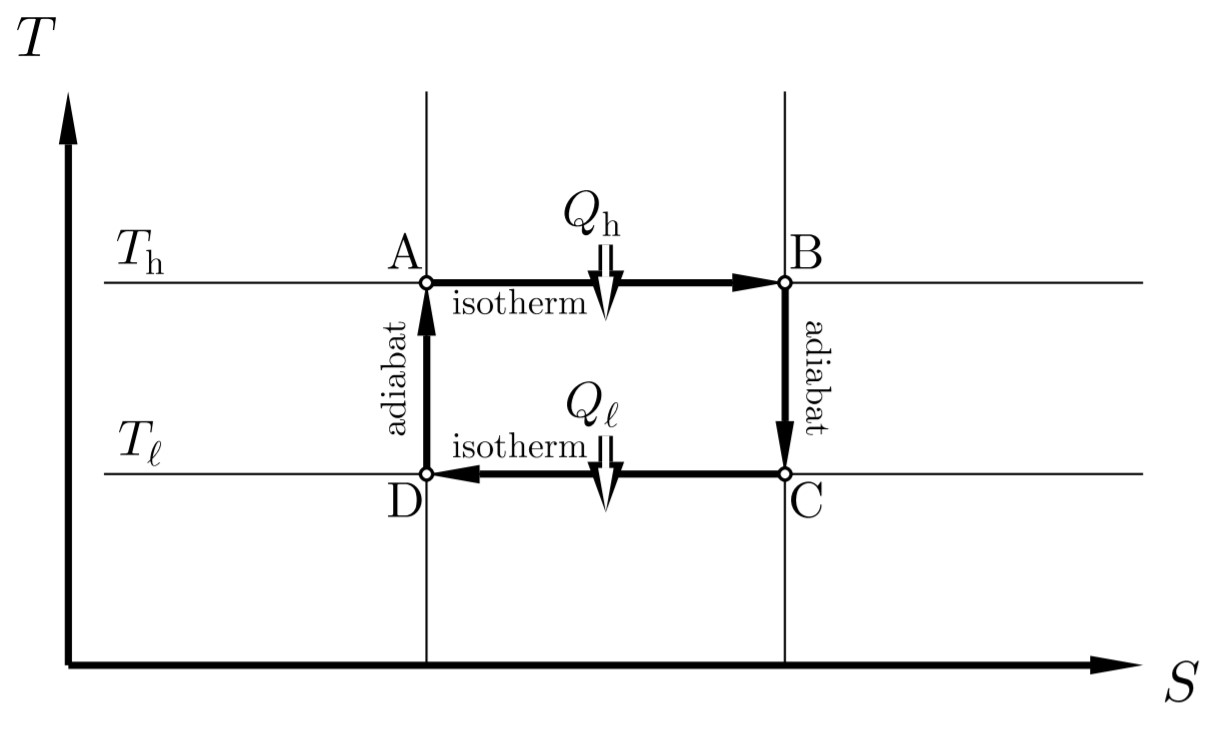
\includegraphics[width=8cm]{adia_ts}
	\centering
	\caption{A T-S plot of the Carnot cycle. 
	$S$ here remains an undefined quantity that we assert is a function of $pV^{\gamma}$ for now.
}
	\label{fig:adia_ts}
\end{figure}
\begin{defi}[Heat engine]
An \textbf{engine} is a system operating a \textit{cyclic} process that converts heat into work. 
\end{defi}
An example of a heat engine is the Carnot engine. 
\begin{defi}[Carnot engine]
A \textbf{Carnot engine} runs on the Carnot cycle, consisting of two heat reservoirs of different temperatures, as shown in \Cref{fig:adia_pv,fig:adia_ts}. 
Thermodynamically, it consists of four alternating reversible isotherms and adiabats. 
Heat only enters and leaves on the isotherms whereas work is performed on all four segments. 
\end{defi}

\begin{thrm}[Work done by Carnot engine]
As this process is cyclic, we can conclude that 
\begin{equation}
W=Q_h-Q_l
\end{equation}
We can write down the governing equations for each segment: 
\begin{subequations}
\begin{align}
A\rightarrow B&:Q_h=RT_h\ln\frac{V_B}{V_A}, \label{car1}\\
B\rightarrow C&:\left(\frac{T_h}{T_l}\right)=\left(\frac{V_C}{V_B}\right)^{\gamma-1}, \label{car2}\\
C\rightarrow D&:Q_l=-RT_l\ln\frac{V_D}{V_C}, \label{car3}\\
D\rightarrow A&:\left(\frac{T_l}{T_lh}\right)=\left(\frac{V_A}{V_D}\right)^{\gamma-1}. \label{car4} 
\end{align}
\end{subequations}
\Cref{car2,car4} lead to
\begin{equation}
\label{car5}
\frac{V_B}{V_A}=\frac{V_C}{V_D}, 
\end{equation}
and dividing \Cref{car1} by \Cref{car3} and substituting in \Cref{car5} gives 
\begin{equation}
\label{carnot_relation}
\frac{Q_h}{Q_l}=\frac{T_h}{T_l}
\end{equation}
\end{thrm}

\begin{defi}[Efficiency]
\begin{equation}
\eta=\frac{W}{Q_h}
\end{equation}
\end{defi}

\begin{lemma}[Efficiency of Carnot engine]
\begin{equation}
\begin{aligned}
\eta_{Carnot}&=\frac{Q_h-Q_l}{Q_h}, \\
\eta_{Carnot}&=\frac{T_h-T_l}{T_h}, \\
&=1-\frac{T_l}{T_h}.  
\end{aligned}
\end{equation}
\end{lemma}

\begin{thrm}[Carnot's theorem]
Carnot's Theorem states that, of all the heat engines working between two given temperatures, none is more efficient than a Carnot engine. 
\end{thrm}

\begin{proof}
We prove the theorem by contradiction. 
Suppose there exists engine E such that $\eta_E>\eta_{Carnot}$. 
Engine E and a Carnot engine running in reverse (having work done \textit{to} it) are connected together with two heat reservoirs at $T_h$ and $T_l$ respectively as shown in \Cref{fig:carnot_thm}. 
We have, 
\begin{equation}
\label{carnot_0}
\begin{aligned}
\frac{W}{Q_h'}&>\frac{W}{Q_h}, \\
Q_h&>Q'_h. 
\end{aligned}
\end{equation}
We also have, 
\begin{equation}
\label{eq:carnot_thm}
\begin{aligned}
W=Q'_h-Q'_l&=Q_h-Q_l, \\
Q_h-Q'_h&=Q_l-Q'_l. 
\end{aligned}
\end{equation}
Now \Cref{eq:carnot_thm} means this compound engine is extracting a positive (due to \Cref{carnot_0}) amount of energy from the low temperature reservoir and dumping the same amount of energy into the high temperature reservoir. 
This is in direct violation of \Cref{L2} and therefore E cannot exist. 
\end{proof}

\begin{figure}[!htbp]
	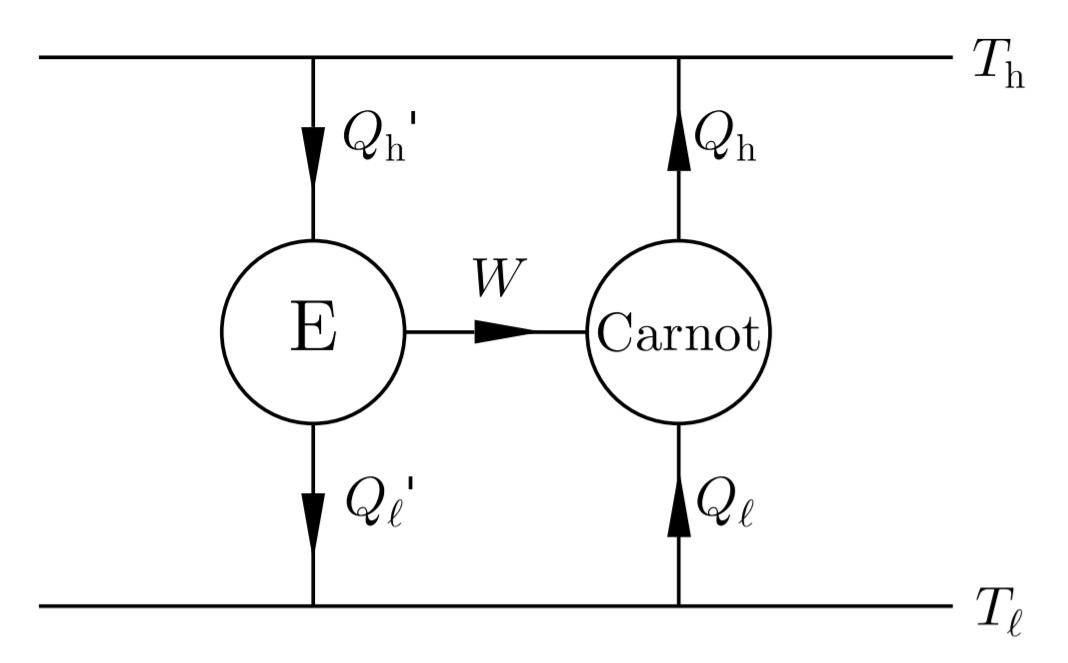
\includegraphics[width=8cm]{carnot_thm}
	\centering
	\caption{Proof of optimality of Carnot engine.}
	\label{fig:carnot_thm}
\end{figure}

\begin{coro}
All reversible engines working between two temperatures have the same efficiency $\eta_{Carnot}$
\end{coro}
\begin{proof}
Suppose there is another reversible engine R such that $\eta_R\leq\eta_{Carnot}$. We run it in reverse and connect to a forward Carnot engine. This arrangement will again transfer heat from the cold reservoir to the hot one, \textit{unless} they have the same efficiency. 
\end{proof}

\begin{prop}[Equivalence of Clausius and Kevin statements]
If a system violates Kelvin's statement of the second law, it also violates Clausius's statement, and \textit{vice versa}. 
\end{prop}
\begin{proof}
As shown in \Cref{kelvin_vio}, by connecting a Kelvin violator, which extracts $Q'_h$ and outputs the same amount of $W$, to a Carnot engine, which extracts $Q_l$, and outputs $Q_h$, we arrive at the same conclusion that this setup violates Clausius statement. 

\begin{figure}[!htbp]
	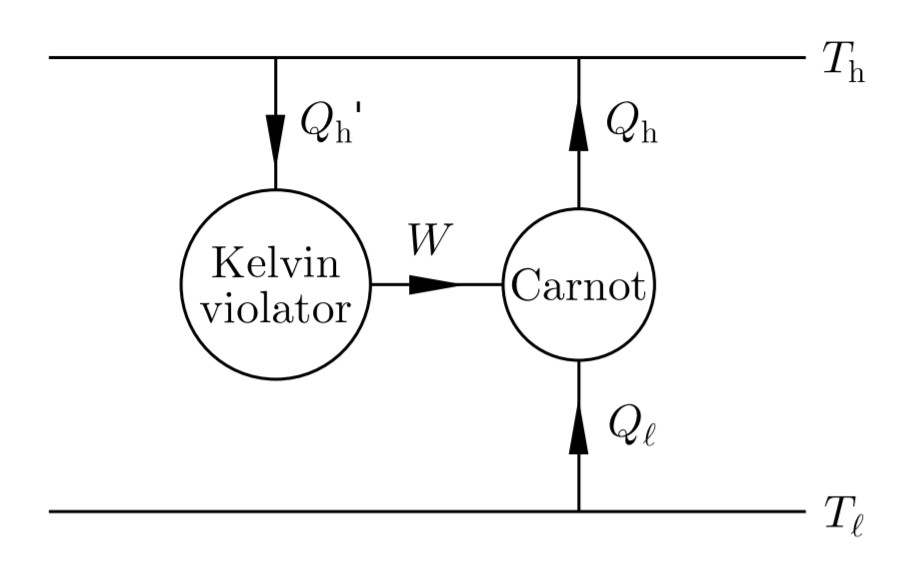
\includegraphics[width=8cm]{kev_vio}
	\centering
	\caption{}
	\label{kelvin_vio}
\end{figure}
\begin{figure}[!htbp]
	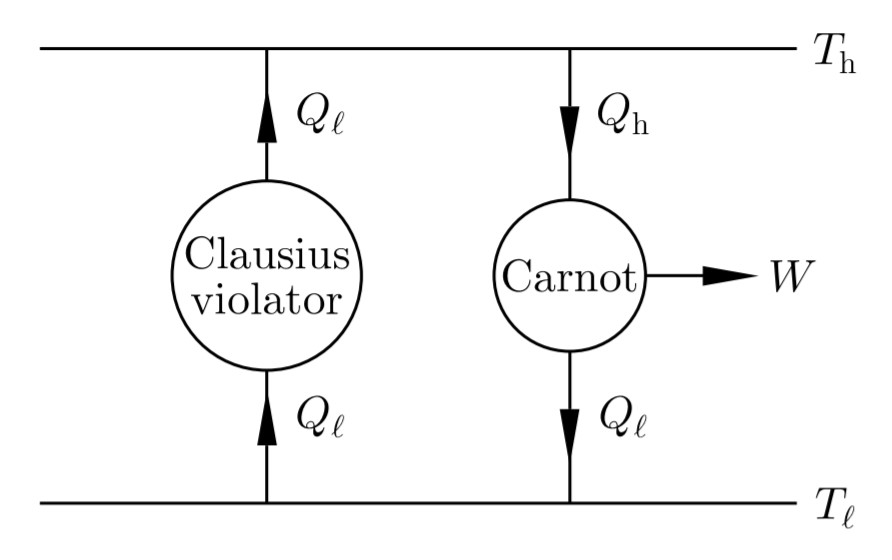
\includegraphics[width=8cm]{clau_vio}
	\centering
	\caption{}
	\label{clau_vio}
\end{figure}

Now, in \Cref{clau_vio} we connect a Clausius violator, transferring $Q_l$ from cold to hot reservoir, 
and a Carnot engine, operating forward. 
The net action of the setup is to convert $Q_h-Q_l$ completely into work, 
hence violating Kelvin's statement.
\end{proof}

\subsubsection{Clausius' theorem}
Consider a Carnot cycle. Heat is \textit{not} conserved around a cycle, however \Cref{carnot_relation} states the important result that 
\begin{equation}
\frac{Q_h}{Q_l}=\frac{T_h}{T_l}, 
\end{equation}
and so we are inspired to define $\Delta Q_{rev}$ as the heat entering the system at each segment, and therefore we have 
\begin{equation}
	\sum_{cycle}\frac{\Delta Q_{rev}}{T}=\frac{Q_h}{T_h}+\frac{\left(-Q_l\right)}{T_l}=0, 
\end{equation}
which means $\Delta Q_{rev}/T$ sums to zero around the cycle. Replcing the sum by an integral we could write 
\begin{equation}
	\oint \frac{\indiff Q_{rev}}{T}=0
\end{equation}
for the Carnot cycle. 

To make a generalised case, we consider a general thermodynamic cycle in \Cref{gen_cyc}(a), where heat $\indiff Q_i$ enters (or leaves, depends on the sign taken up) at a point in the cycle. 
At this point the system is connected to a reservoir at $T_i$. The total work extracted from the cycle is 
\begin{equation}
\Delta W = \sum_{cycle}\indiff Q_i. 
\end{equation}
\begin{figure}[!htbp]
	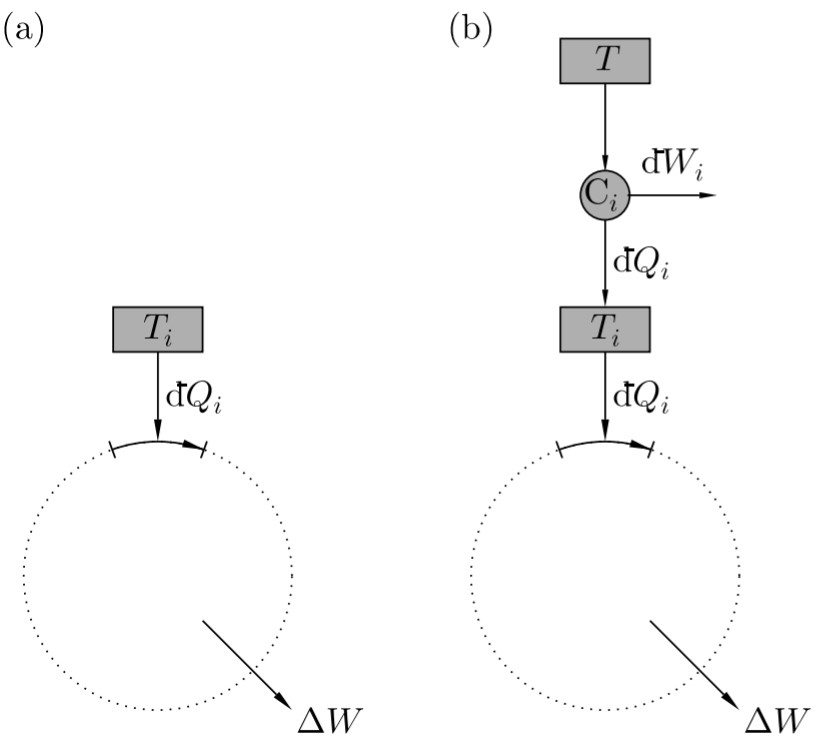
\includegraphics[width=8cm]{gen_cyc}
	\centering
	\caption{}
	\label{gen_cyc}
\end{figure}
Now suppose, as in \Cref{gen_cyc}(b) that all the $\indiff Q_i$ is provided by Carnot engine(s) $C_i$, 
whose input reservoir is fixed at $T$ and output reservoir is the variable $T_i$. 
The Carnot engine itself outputs work $\indiff W_i$. 
We know, for a Carnot engine, 
\begin{equation}
\begin{aligned}
\frac{\text{heat to reservoir at}\ T_i}{T_i}&=\frac{\text{heat from reservoir at}\ T}{T} \\
\frac{\indiff Q_i}{T_i}&=\frac{\indiff Q_i + \indiff W_i}{T} \\
\indiff W_i&=\indiff Q_i \left(\frac{T}{T_i}-1\right). 
\end{aligned}
\end{equation}
For the system to not violate Kelvin's statement of second law, \ie not to convert all the heat into work, as there is no output heat, we must require that 
\begin{equation}
\begin{aligned}
\text{output work}&\leq0 \\
\sum_{cycle}\indiff W_i + \Delta W &\leq 0 \\
T\sum_{cycle}\frac{\indiff Q_i}{T_i}&\leq 0 \\
\oint\frac{\indiff Q}{T}&\leq0, 
\end{aligned}
\end{equation}
which is the \textbf{Clausius inequality}. 

\begin{thrm}[Clausius's theorem]
\label{clau_thrm}
For any closed cycle, $\oint \frac{\indiff Q}{T}\leq0$, where equality necessarily holds for a reversible cycle. 
\end{thrm}

\subsection{Entropy}
We now are in position to introduce the thermodynamic quantity of entropy. 
According to \Cref{clau_thrm}, the integral 
\begin{equation}
\int_A^B \frac{\indiff Q_{rev}}{T}
\end{equation}
is path independent. Therefore the quantity $\indiff Q_{rev}/T$ is an \textit{exact} differential. 
\begin{defi}[Entropy]
Entropy is defined as a state function
\begin{equation}
\dif S=\frac{\indiff Q{rev}}{T}. 
\end{equation}
\end{defi}

\begin{prop}[Adiabatic entropy change]
For an adiabatic process (\textit{defined} as an adiathermal reversible process), 
we have
\begin{equation}
\dif Q_{rev}=0. 
\end{equation}
Hence an adiabatic process involves no change in entropy, \ie isoentropic. 
\end{prop}

\begin{thrm}[Entropy inequality]
Consider a cycle with a reversible and an irreversible segment, 
\Cref{clau_thrm} gives that 
\begin{equation}
\begin{aligned}
	\oint\frac{\indiff Q}{T}&\leq0 \\
	\int^B_A\frac{\indiff Q}{T}+\int^A_B\frac{\indiff Q_{rev}}{T}&\leq0 \\
	\int^B_A\frac{\indiff Q}{T}&\leq\int^B_A\frac{\indiff Q_{rev}}{T} \\
	\dif S = \frac{\indiff Q_{rev}}{T}&\geq\frac{\indiff Q}{T}. 
\end{aligned}
\end{equation}
If we consider a thermally isolated system, \ie $\indiff Q=0$, we then have
\begin{equation}
	\dif S \geq0. 
\end{equation}
\end{thrm}

Now we are in a position to revisit the first law: 
\begin{thrm}[The first law]
For a reversible change only, we have that 
\begin{subequations}
\begin{align}
\indiff Q&=T\dif S \\
\indiff W&=-p\dif V. 
\end{align}
\end{subequations}
For an irreversible change $\indiff Q\leq T\dif S$ and $\indiff Q\geq-p\dif V$, but we \textit{always} have that 
\begin{equation}
\dif U=T\dif S-p\dif V. 
\end{equation}
\end{thrm}
We observe that $S$ and $V$ are the \textbf{natural variables} of $U$, 
and that they are both \textit{extensive}. 
$p$ and $T$ however are \textit{intensive} and behave somewhat like \textit{forces}
\section{Mathematical methods}
\subsection{Legendre transforms}
This subsection is adapted from \cite{lgd_wiki,lgd_paper} and Appendix F of \cite{dill}. \\
Legendre transform, as we will see, is really just a long way to say 'In a right-angled triangle, the slope (tangent) times the adjacent side equals the opposite side'. \\
For a function $F(x)$, we have all the information of the function $F$ stored as ordered pairs of values $(x_i,F(x_i))$. There are many ways to store the same information of the function, one of which is through the gradient. For a function $F$ whose second derivative is always positive, \ie $F$ is monotonously increasing, the gradient $s(x)=\diff {F(x)}/x$ is one-one to $x$, therefore we can invert it to get a single-valued function $x(s)$. 
\begin{figure}[!htbp]
	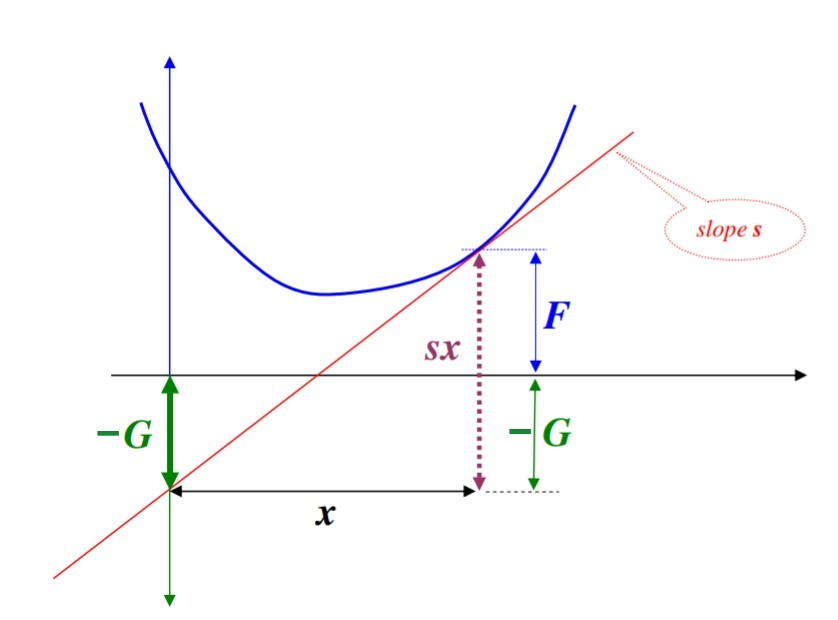
\includegraphics[width=8cm]{legendre1}
	\centering
	\caption{Sometimes the opposite sign convention for $G$ is used to confer more symmetry.}
	\label{legendre1}
\end{figure}
\begin{defi}[Legendre transform]
As shown in \Cref{legendre1}, we are inspired to write
\begin{equation}
sx=F+(-G).
\end{equation}
Rearranged and showing explicitly the functional relationships, 
\begin{equation}
\label{legendre}
G(s)=F(x(s))-sx(s),
\end{equation}
with $-G(s)$ (note the negative sign) known as the Legendre transform of $F(x)$.
This is, at the root of it, just the geometrical statement at the beginning of the section. 
\end{defi}
\begin{prt}[Inverse]
The inverse of the Legendre transform is the starting function, \ie the Legendre transform is its own inverse. We can see this by starting with 
\begin{equation}
y(s)=-\diff Gs
\end{equation}
and inverting the monotonic function $y(s)$ to $s(y)$. 
We then construct the Legendre transform, $H(y)$ of $G(s)$:
\begin{equation}
\begin{aligned}
H(y)&=G(s(y))-ys(y)\\
G&=H-sy
\end{aligned}
\end{equation}
Comparison with \Cref{legendre} reveals that we can identify $\{H,y\}$ with $\{F,x\}$.
This gives us a recursive relation
\begin{subequations}
\begin{align}
s(x)&=\diff Fx \label{lgd_1}\\
x(s)&=-\diff Gs. \label{lgd_2}
\end{align}
\end{subequations}
\Cref{lgd_2} can actually be obtained by differentiating \Cref{legendre}:
\begin{equation}
\diff{G(s)}{s}=\diff{F(x(s))}{s}-x(s)-s\diff xs=-x(s)-s\diff xs+\diff Fx\diff xs=-x(s).
\end{equation}
The symmetric is perhaps best displayed as 
\begin{equation}
\label{lgd_symm}
-G(s)+F(x)=sx.
\end{equation}
Make no mistake here - there is only one independent variable: \textit{either} $x$ \textit{or} $s$, with the other variable written as a function of it. The pair of variables $x$ and $s$ are called \textit{conjugate} variables. 
\end{prt}
\begin{prt}[Extrema]
Remembering that $F$ is defined upwards positive and $G$ downwards positive, as shown in \Cref{legendre1}, we have
\begin{subequations}
\begin{align}
F_{\text{min}}&=-G(0)\\
-G_{\text{min}}&=-F(0).
\end{align}
\end{subequations}
This can be expressed in a more symmetrical form, with the RHS in \Cref{lgd_symm} vanishing in either case: 
\begin{equation}
-G(0)+F(x_{\text{ext}})=0\ \ \ \text{and}\ \ \ -G(s_{\text{ext}})+F(0)=0.
\end{equation}
\end{prt}
We now look at functions of more than one variables, for example, $F(x,y)$. 
We require that $F$ is convex in $x$ for all $y$ and vice versa.
The differential is 
\begin{equation}
\dif F=\diffp Fx \dx + \diffp Fy \dif y\equiv p\dx+v\dif y,
\end{equation}
where $\{p,x\}$ and $\{v,y\}$ are conjugate pairs of variables, and $p$ and $v$ can be understood as the gradient in the two basis vector directions. \\
The Legendre transform aims, again, to swap one variable for its conjugate variable, say $x$ for $p$. 
So essentially we `flatten' a multivariate function into one dimension and the Legendre transform is 
\begin{equation}
G(p,y)\equiv F\bigr(x(p),y\bigl)-px(p).
\end{equation}
We see in the differential form that indeed the independent variable $x$ is switched into $p$:
\begin{equation}
\dif G=\dif F-p\dx-x\dif p=-x\dif p+v\dif y.
\end{equation}
We can identify
\begin{subequations}
\begin{align}
x&=-\diffp Gp \\
v&=\diffp Gy.
\end{align}
\end{subequations}
\begin{wex}
\label{wex_enthalpy}
The internal energy is
\begin{equation}
U=U(S,V,\bvec{N}), 
\end{equation}
with total differential given by
\begin{equation}
dU=T\dif S-P\dif V+\sum \mu_i\dif N_i
\end{equation}
We know from \Cref{diff_p} that $-p$ (again note the negative sign) and $V$ are \textit{defined} by the foundamental thermodynamic equations to be conjugate variables. 
We therefore wish to define a new quantity $H=H(S,p,\bvec{N})$ via a Legendre transform:
\begin{equation}
H(S,p,\bvec{N})\equiv U+pV.
\end{equation}
We can immediately recover from the properties of Legendre transforms that
\begin{subequations}
\begin{align}
V&=\diffp Hp\\
T&=\diffp HS\\
\mu_i&=\diffp{H}{N_i},
\end{align}
\end{subequations}
where subscripts are omitted for clarity. \\
The function $H$ being a Legendre transform of $U$, encodes the exact same information as $U$ but are easier to work with in situations where pressure is constant, as the total differential simplifies. 
\end{wex}
\subsection{Euler-Maclaurin formula}
This is adapted from \cite{emform}. \\
We wish to approximate a sum 
\begin{equation}
S(n)=\sum^{n}_{k=0}f(k)
\end{equation}
by an integral of the form
\begin{equation}
\label{sigman}
\sigma(n)=\int^n_0 f(x)\dx. 
\end{equation}
But this is inaccurate for fast changing sums and it'll be more accurate to 
approximate behaviour of the function near each integer value, which is to say 
that we write the integral this way
\begin{equation}
\sigma(n)=\int^1_0[f(0+x)+f(1+x)+f(2+x)+\cdots+f(n-1+x)]\dx.
\end{equation}
We approximate the behaviour of the function about each integer with a Taylor 
series expansion:
\begin{equation}
f(k+x)=\sum^{\inf}_{j=0}\frac{f^{(j)}(k)}{j!}x^j, 
\end{equation}
whose integral from $0$ to $1$ is 
\begin{equation}
\int^1_0 f(k+x)\dx=\sum^{\inf}_{j=0} \frac{f^{(j)}(k)}{(j+1)!}
\end{equation}
So,
\begin{equation}
\label{sigman2}
\sigma(n)=\sum^{\inf}_{m=0}\frac{S^{(m)}}{(m+1)!}.
\end{equation}
Taking derivative of \Cref{sigman2} we have 
\begin{equation}
\sigma^{(j)}(n)
\end{equation}

\subsection{Homogeneous functions}
\label{homofun}
A polynomial
\begin{equation}
  a_0+a_1x+a_2x^2+\dots+a_nx^n
\end{equation}
is of degree $n$. A polynomial is said to be homogeneous of degree $n$ if all its terms are of the same degree $n$, for example,
\begin{equation}
  x^2+5xy+13y^2
\end{equation}
is homogeneous of degree $2$. The same idea can be extended to functions: if for arbitrary $\lambda$
\begin{equation}
  f(\lambda x)=\lambda^nf(x)
\end{equation}
$f$ is said to be homogeneous of degree $n$ in the variable $x$, and
\begin{defi}[Intensive and extensive variables]
Intensive functions are homogeneous of degree zero and extensive functions are homogeneous of degree one.
\end{defi}
Now consider 
\begin{equation}
  S=S(U,V,n)
\end{equation}
physically, entropy is extensive, so we can write
\begin{equation}
  S(\lambda U,\lambda V,\lambda n)=\lambda S(U,V,n)
\end{equation}
If we choose $\lambda=1/n$ we can write
\begin{equation}
  S(\tfrac{U}{n},\tfrac{V}{n},1)\equiv S_m(U_m,V_m)=\frac{1}{n}S(U,V,n)
\end{equation}
so
\begin{equation}
  nS_m(U_m,V_m)=S(U,V,n)
\end{equation}
This illustrates why $\lambda$ is known as the \emph{scaling function}.

\section{Free energies}
\label{free_energy}
This section is adapted from \cite{dill}. \\
In laboratory conditions, microscopic, extensive quantities such as $S$, $U$ and $\bvec{N}$ is difficult to keep track of at boundaries of systems. 
Instead we can control and keep track of macroscopic, intensive quantites such as $p$ and $T$. 
This makes the use of $U(S,V,\bvec{N})$ or $S(U,V,\bvec{N})$ rather cumbersome. 
However, the second law still applies and as such we can devise new extrumum principles to find conditions of equilibrium. 

\subsection{Helmholtz free energy}
\subsubsection{Inspiration}
\label{A_insp}
Imagine a test tube in a water bath at a fixed temperature $T$, which act as a thermal reservoir. Therefore we need to find a function $A$ whose natural variables are $(T,V,\bvec{N})$ for us to construct a new extremum principle. \\
Now assume that the combined heat bath-test tube system isolated from its surroundings, equilibrium is predicted by the state of maximum entropy $S(U,V,\bvec{N})$. Any change towards equilibrium must have that
\begin{equation}
\label{sbathstt}
\dif S_{\text{combined system}}=\dif S_{\text{bath}}+\dif S_{\text{test tube}}\geq0.
\end{equation}
Since the combined system is isolated, 
\begin{equation}
\label{ubathutt}
\dif U_{\text{bath}}+\dif U_{\text{test tube}}=0.
\end{equation}
The fundamental equation gives 
\begin{equation}
\dif S_{\text{bath}}=\left(\frac{1}{T}\right)\dif U+\left(\frac{p}{T}\right)\dif V-\left(\frac{\mu}{T}\right)\dif N=\left(\frac{1}{T}\right)\dif U_{\text{bath}}=-\frac{\dif U_{\text{test tube}}}{T}, 
\end{equation}
where the second equality comes from \Cref{ubathutt}. Applying \Cref{sbathstt} further results in
\begin{subequations}
\begin{align}
\dif S_{\text{test tube}}-\frac{\dif U_{\text{test tube}}}{T}&\geq0\\
\dif U_{\text{test tube}}-T\dif S_{\text{test tube}}&\leq0, 
\end{align}
\end{subequations}
where we have successfully obtained a relation only in terms of the test tube quantities. We therefore define 
\begin{defi}[Helomoltz free energy]
\begin{equation}
A\equiv U-TS, 
\end{equation}
with differential 
\begin{equation}
\dif A=\dif U-T\dif S-S\dif T=\dif U-T\dif S\ \ \ \text{at constant temperature.}
\end{equation}
Therefore we see that Helmholtz free energy is essentially the amount of reversible work obtainable from an isothermal and isochoric system:
\begin{equation}
\begin{aligned}
\dif A&=\indiff Q+\indiff W-T\dif S\\
&=\indiff W, 
\end{aligned}
\end{equation}
where we assumed reversibility, which extracts most amount of work.
\end{defi}
\begin{prt}[Condition of equilibrium]
We can see that the condition in \Cref{sbathstt} is fulfiled when 
\begin{equation}
(\dif A)_T\leq0. 
\end{equation}
This means that equilibrium is reached when $A$ is at a minimum.
\end{prt}
\begin{prt}[Fundamental equation]
\begin{equation}
\dif A=-S\dif T-p\dif V+\sum_{j=1}^M\mu_j\dif N_j
\end{equation}
And we can trivially obtain more definitions:
\begin{subequations}
\begin{align}
S&=-\diffp FT[V,\bvec{N}]\\
p&=-\diffp FV[T,\bvec{N}]\\
\mu_j&=\diffp{A}{N_j}[V,T,N_{i\neq j}]. 
\end{align}
\end{subequations}
On the surface this definition seems strange because we need to hold $T$ and $V$ constant and we're only left with the chemical potential term. It is true that if we're looking at a one-component non-reacting system, if we fix $T$ and $V$, no change can take place. But in a multi-component, reacting mixture with fixed $T$ and $V$ we have 
\begin{equation}
\dif A=\sum_{j=1}^M\mu_j\dif N_j
\end{equation}where $A$ can depend on $T$ and $V$ in the \textit{equation of state}, we have the chemical potential terms in the differentials, which changes to minimise the entropy. The following two examples illustrates this idea.
\end{prt}
\subsubsection{A microscopic look at Helmholtz I: Dimerisation}
Suppose $N=2$ gas particles are contained in a test tube of $V$ lattice sites in a row at $T$. We ask under what conditions will the two associate into a dimer. We compute the free energies of monomer and dimer states and compare them. \\
\textbf{Dimers: }Suppose when two monomer sit on adjacent sites a 'bond energy' $U=-\epsilon$ is additionally introduced. \\
Within $V$ sites, multiplicity for a dimer is 
\begin{equation}
W_{\text{d}}=V-1\approx V. 
\end{equation}
The Helmholtz free energy is then given as 
\begin{equation}
A_{d}=U_{d}-TS_{d}=-\epsilon-kT\ln V.
\end{equation}
\textbf{Monomers: }There is no energy of interaction, and the multiplicity is 
\begin{equation}
W_{m}=W_{\text{total}}-W_{d}=\frac{V!}{(2!)(V-2)!}-(V-1)=\left(\frac{V}{2}-1\right)(V-1)\approx\frac{V^2}{2}.
\end{equation}
So the free energy is
\begin{equation}
A_m=-kT\ln\left(\frac{V^2}{2}\right).
\end{equation}
Temperature at which both are equally stable is, after some algebra
\begin{equation}
T_0=\frac{\epsilon}{k\ln(V/2)}.
\end{equation}
Had we only maximised entropy we would conclude that the dimers will never even form, hence missing out on the significant role energy plays at lower temperatures here. 
\subsubsection{A microscopic look at Helmholtz II: Polymer collapse}
\label{polymer_collapse}
\begin{figure}[H]
	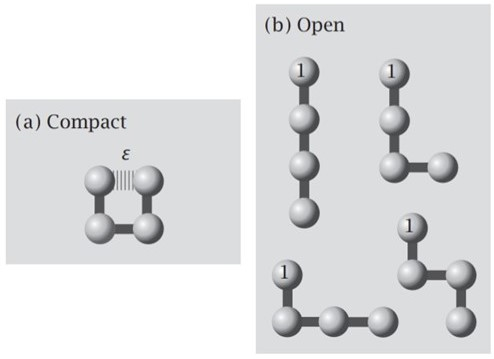
\includegraphics[width=8cm]{polymer_collapse}
	\centering
	\caption{The two energy levels.}
	\label{fig:polymer_collapse}
\end{figure}
Consider a two-dimensional model polymer with four monomers in a closed test tube solution in a bath at $T$ and the ends of the polymer are attracted to each other by $U=-\epsilon$. The multiplicity is $1$ as only one conformation can result in the close-ring polymer. The open-ring state has $4$ other multiplicities. We compute the free energies:
\begin{subequations}
\begin{align}
A_c&=-\epsilon-kT\ln 1=-\epsilon\\
A_o&=-kT\ln 4.
\end{align}
The collapse temperature $T_0$ is given as
\begin{equation}
T_0=\frac{\epsilon}{k\ln 4}.
\end{equation}
\end{subequations}
We note that for this process, 
\begin{subequations}
\begin{align}
\Delta F_{\text{collapse}}&=-\epsilon+kT\ln 4 \\
\Delta U_{\text{collapse}}&=-\epsilon\\
\Delta S_{\text{collapse}}&=-k\ln 4
\end{align}
\end{subequations}
As no volume change is involved, in a reversible process no work is done and $\Delta U=-\epsilon$ and the process is exothermic at all temperature. 
\subsection{Enthalpy}
The enthalpy is most commonly obtained as a Legendre transform of $U$ as explained in \Cref{wex_enthalpy}. We can write out the total differential:
\begin{equation}
\dif H=T\dif S+V\dif P+\sum\mu_j\dif N_j.
\end{equation}
At constant pressure, with a non-reacting mixture, we can write 
\begin{equation}
\dif S=\frac{\dif H}{T}.
\end{equation}
By way of the argument used in \Cref{A_insp}, we introduce two systems $A$ and $B$, 
with $A$ being an open test tube and $B$ the surroundings, acting as a pressure reservoir. Any change towards \eqm will have 
\begin{equation}
\dif S_{A+B}=\dif S_A+\dif S_B\geq0.
\end{equation}
Because $B$ is also a temperature reservoir, we write 
\begin{equation}
\dif S_B=-\frac{\indiff Q_A}{T}.
\end{equation}
Combined, we have
\begin{equation}
\dif S_A-\frac{\indiff Q_A}{T}\geq0.
\end{equation}
Under constant pressure we have
\begin{equation}
\dif H=\dif U+p\dif V-V\dif p=\indiff Q-p\dif V+p\dif V-V\dif p=\indiff Q, 
\end{equation}
and as such
\begin{equation}
T\dif S_A-\dif H\geq0. 
\end{equation}
For tending to equilibrium inside $A$, we require that
\begin{equation}
\dif S_A\geq0,
\end{equation}
therefore 
\begin{equation}
\frac{\indiff Q_A}{T}\leq0.
\end{equation}
So finally we have that
\begin{equation}
\dif H\leq0
\end{equation}
for processes to tend to equilibrium at constant pressure.
\subsection{Gibbs free energy}
To get a function that is minimised at equilibrium at constant pressure and temperature, we perform a Legendre transform on $H(S,p,\bvec{N})$ to get $G(T,p,\bvec{N})$, nothing that $T$ and $S$ are a conjugate pair and the usual sign convention applies:
\begin{equation}
G(T,p,\bvec{N})=H-TS.
\end{equation}
The total differential is given as 
\begin{equation}
\dif G=-S\dif T+V\dif p+\sum\mu_j\dif N_j.
\end{equation}
At constant pressure and temperature, 
\begin{equation}
\dif G=\dif H-T\dif S=\indiff Q-T\dif S.
\end{equation}
Invoking Clausius theorem we can show the equilibirum condition, but to do so explicitly, we use the second law, for 
\begin{equation}
\dif S_{A+B}=\dif S_A+\dif S_B=\dif S_A-\frac{\indiff Q_A}{T}\geq0, 
\end{equation}
under constant pressure and temperature, this becomes
\begin{equation}
\begin{aligned}
T\dif S_A-\dif H_A&\geq0\\
(\dif G)_{p, T}&\leq0.
\end{aligned}
\end{equation}
Therefore $G$ is minimised at equilibrium. \\
It is called `free energy' because it shows how much non-mechanical work can be extracted, which is important in chemistry and biology, again we assume constant pressure and temperature: 
\begin{subequations}
\begin{align}
\dif G&=\dif U+p\dif V-T\dif S\\
&=T\dif S-p\dif V+\indiff W_x+p\dif V-T\dif S\\
&=\indiff W_x, 
\end{align}
where we assume the process is reversible, and the $x$ subscript means other forms of work like electrical work.
\end{subequations}
\subsection{More on thermodynamic functions}
\subsubsection{Functional dependencies}
Below we give a summary of the fundamental functions. \\
\begin{table}[H]
\resizebox{\textwidth}{!}{
\begin{tabular}{c c l l l}
\hline
Function & Extremum at eqm & Fundamental equation & Definition & Useful for \\ \hline
$U(S,V,\bvec{N})$ & Minimum & \(\displaystyle \dif U=T\dif S-p\dif V+\sum\mu_j\dif N_j\) &\ &\ \\ 
$S(U,V,\bvec{N})$ & Maximum & \(\displaystyle \dif S=\lf(\frac{1}{T}\rt)\dif U+\lf(\frac{p}{T}\rt)\dif V+\sum\lf(\frac{\mu_j}{T}\rt)\dif N_j\)&\ &\ \\ 
$H(S,p,\bvec{N})$ & Minimum & \(\displaystyle \dif H=T\dif S+V\dif p+\sum\mu_j\dif N_j\)& $H\equiv U+pV$ & Const $S$ and $p$, $\dif H=\dif U$ \\ 
$A(T,V,\bvec{N})$ & Minimum & \(\displaystyle \dif A=-S\dif T-p\dif V+\sum\mu_j\dif N_j\)& $A\equiv U-TS$ & Const $T$ and $V$, $\dif A=\indiff W$\\ 
$G(T,p,\bvec{N})$ & Minimum & \(\displaystyle \dif G=-S\dif T+V\dif p+\sum\mu_j\dif N_j\)&$G\equiv H-TS\equiv A+pV$ & Const $T$ and $p$, $\dif G=\indiff W_x$\\ \hline
\end{tabular}
}
\end{table}
We should be aware that, for example the function $U$ in $A=U-TS$ is not $U(S,V,\bvec{N})$ but instead takes on the arguments of $A$ such that $U=U(T,V,\bvec{N})$. 
This is why minimising $U(T,V,\bvec{N})$ or maximising $S(T,V,\bvec{N})$ individually does not give us \eqm but only their sum in this specific functional form, when minimised, gives equilibrium. \\
We illustrate this idea by considering 
\begin{equation}
G(T,p,\bvec{N})=H(T,p,\bvec{N})-TS(T,p,\bvec{N}).
\end{equation}
$H$ and $S$ here are non-fundamental functions, but they are useful in that they can be conveniently measured and calculated. Now because at constant pressure, 
\begin{equation}
C_p=\lf(\frac{\indiff Q}{\dif T}\rt)_p=\diffp HT[p]=T\diffp ST[p],
\end{equation}
we can write that
\begin{subequations}
\begin{align}
\Delta H(T,p)&=\int^{T_B}_{T_A}C_p(T)\dif T \\
\Delta S(T,p)&=\int^{T_B}_{T_A}\frac{C_p(T)}{T}\dif T.
\end{align}
\end{subequations}
From a series of constant-pressure heat capacity experiments one can obtain $G(T,p)$. \\
From constant-volume heat capacity experiments one can similarly obtain $A(T,V)=U(T,V)-TS(T,V)$ since we know that at constant volume,
\begin{equation}
C_V=\diffp UT[V]=T\diffp ST[V],
\end{equation}
we can write 
\begin{subequations}
\begin{align}
\Delta U(T,V)&=\int^{T_B}_{T_A}C_V(T)\dif T \\
\Delta S(T,V)&=\int^{T_B}_{T_A}\frac{C_V(T)}{T}\dif T.
\end{align}
\end{subequations}
\subsubsection{Non-standard states}
We can further write, for ideal mixtures,
\begin{equation}
\begin{aligned}
  \dif G&=\frac{nRT}{p}\dif p\\
  \int^{p_2}_{p_1}\dif G&=\int^{p_2}_{p_1}\frac{nRT}{p}\dif p\\
  G(p_2)-G(p_1)&=nRT\ln\frac{p_2}{p_1}\\
  G(p)&=G^{\circ}+nRT\ln\frac{p}{p^{\circ}}
\end{aligned}
\end{equation}
For ideal gases, the chemical potential is the molar Gibbs energy, so we can always write
\begin{equation}
  \mu_i(p_i)=\mu_i^{\circ}+RT\ln\frac{p_i}{p^{\circ}}
\end{equation}
and a parametric ($\mu(p)\rightarrow\mu(c(p))$) substitution gives
\begin{equation}
  \mu_i(c_i)=\mu_i^{\circ}+RT\ln\frac{c_i}{c^{\circ}}
\end{equation}
And for the generic reaction
\begin{equation}
  \ch{$\nu$_AA + $\nu$_BB <=> $\nu$_MM + $\nu$_NN}
\end{equation}
with some algebra we get
\begin{equation}
\label{stdgibbsp}
  \Delta_rG^{\circ}=-RT\ln K_p
\end{equation}
and also
\begin{equation}
\label{stdgibbsc}
  \Delta_rG^{\circ}=-RT\ln K_c
\end{equation}
\subsubsection{Gibbs-Helmholtz equation}
For the function $G/T$, we can always write, with chain rule:
\begin{equation}
  \diffp{}{T}(GT^{-1})=T^{-1}\diffp GT-T^{-2}G
\end{equation}
noting that $\diffp G/T=-S$ by definition, we proceed:
\begin{equation}
\begin{aligned}
  \diffp{}{T}(GT^{-1})&=-ST^{-1}-T^{-2}(H-TS)\\
  &=-\frac{H}{T^2}
\end{aligned}
\end{equation}
where we have derived the
\begin{thrm}[Gibbs-Helmholtz equation]
The equation states that
\begin{equation}
  \diffp{}{T}\lf(\frac{G}{T} \rt)=-\frac{H}{T^2}
\end{equation}
\end{thrm}
From this we can derive the van't Hoff equation
\begin{thrm}[van't Hoff equation]
The equation states that
\begin{equation}
  \diffp{\ln K}{T}=\frac{\Delta_rH^{\circ}}{RT^2}
\end{equation}
\end{thrm}
\begin{proof}
  The free energies in Gibbs-Helmoholtz equation can be replaced by changes (over a reaction):
  \begin{equation}
     \diffp{}{T}\lf(\frac{\Delta_rG^{\circ}}{T} \rt)=-\frac{\Delta_rH^{\circ}}{T^2}
  \end{equation}
  and invoking \cref{stdgibbsp,stdgibbsc} we can write that
  \begin{equation}
    \diffp{}{T}(-R\ln K)=-\frac{\Delta_rH^{\circ}}{T^2}
  \end{equation}
  which rearranges to give the van't Hoff equation.
\end{proof}


\subsection{The Euler and Gibbs-Duhem equations}
\label{eulergibbs}
\subsubsection{The Euler equation}
Referring to \cref{homofun}, we now consider the internal energy, which again is physically an extensive function so we can write\footnote{We use $n$ here for simplicity but this can be easily converted and extended to $\bvec{N}$}
\begin{equation}
  U(\lambda S,\lambda V,\lambda n)=\lambda U(S,V,n)
\end{equation}
using the chain rule, we can write
\begin{equation}
\begin{aligned}
  U(S,V,n)=&\diffp{U}{(\lambda S)}[V,n]\diffp{(\lambda S)}{\lambda}+\diffp{U}{(\lambda V)}[S,n]\diffp{(\lambda V)}{\lambda}+\diffp{U}{(\lambda n)}[S,V]\diffp{(\lambda n)}{\lambda}\\
  =&\diffp{U}{(\lambda S)}[V,n]S+\diffp{U}{(\lambda V)}[S,n]V+\diffp{U}{(\lambda n)}[S,V]n\\
  =&TS-pV+\mu n
\end{aligned}
\end{equation}
This is known as the \textbf{Euler equation}, which relates all sever thermodynamic variables.\par
We can further extend this to the Gibbs free energy, which can be written as 
\begin{equation}
\begin{aligned}
G&=H-TS=U+pV-TS\\
&=TS-pV+\mu n+pV-TS\\
&=\mu n
\end{aligned}
\end{equation}
Which can be simply extended to
\begin{equation}
  G=\sum_i\mu_iN_i
\end{equation}
This \emph{holds true for all homogeneous systems}, which can be non-ideal.
\subsubsection{The Gibbs-Duhem equation}
The Euler equation(s) might looks strange because the total differential has extra terms that are not present in the master equation, and vice versa. We need to realise that the master equation started from the conservation of internal energy, which tells us that $U(S,V,N)$ must be a state function, and we can take the total differential and make the definitions to get
\begin{equation}
  \dif U=T\dif S-p\dif V+\mu\dif N
\end{equation}
The Euler equation on the other hand is a statement of the extensivity of energy. So both expressions are logical and the only way to reconcile the two is to take the extra terms in the differential form of the Euler equation to be zero:
\begin{equation}
\begin{aligned}
  \dif U&=T\dif S+S\dif T-p\dif V-V \dif p+\mu\dif N+ N\dif\mu\\
&=\underbrace{T\dif S-p\dif V+\mu\dif N}_{\dif U}+\underbrace{S\dif T-V\dif p+N\dif\mu}_{=0}
\end{aligned}
\end{equation}
This gives us
\begin{thrm}[The Gibbs-Duhem relation]
The relation states that
\begin{equation}
  S\dif T-V\dif p+\sum_iN_i\dif\mu_i=0
\end{equation}
Which tells us that the three intensive variables are interrelated, and specifying two variables allows us to compute the third.
\end{thrm}
This can be extended to Gibbs free energy, where $G=\sum_i\mu_iN_i$ and the master equation is $\dif G=-S\dif T+V\dif p+\sum_i\mu_i\dif N_i$, and we can conclude
\begin{equation}
  S\dif T-V\dif p+\sum_iN_i\dif\mu_i=0
\end{equation}
Under constant $T$ and $p$, we have
\begin{equation}
  \sum_iN_i\dif\mu_i=0
\end{equation}
which in the more illustrative case of a binary system, gives us
\begin{equation}
  \dif\mu_B=-\frac{N_A}{N_B}\dif\mu_A
\end{equation}
which shows that chemical potentials are functions of the composition $\bvec{N}$.

\section{Maxwell's relations and mixtures}
Before we dive head in to proper statistical thermodynamics, let's push the classical, differntial approach to its logical end. \\
There are many external constraints besides the likes of pressure and volume that we have been discussing, 
for example, a lipid bilayer can change its surface area, and a rubber band its length. We ask the following questions: 
\begin{itemize}
	\item What is the extra degree(s) of freedom, \ie new variables?
	\item What is the fundamental function and what does it depend on?
	\item What is the condition of equilibrium?
	\item Is the process tending to equilibrium driven by entropy or enthalpy or both? 
\end{itemize}
\subsection{Designing a fundamental equation}
\begin{defi}[Conjugate pairs]
We have introduced the idea of conjugate pairs, but we now generalise the definition:\\
For a generalised extensive variable $X_j$, we have the conjugate force-analogue $F_j$that is an intensive variable given as 
\begin{equation}
\label{conj_force}
F_j=\diffp{U}{X_j}[S,V,\bvec{N},X_{i\neq j}].
\end{equation}
\end{defi}
Now to make the new, augmented internal energy function we just introduce the \textit{intensive} variable into the argument to get 
\begin{subequations}
\begin{align}
U&=U(S,V,\bvec{N},\bvec{X})\\
\dif U&=T\dif S-p\dif V+\sum\mu_j\dif N_j+\sum F_j\dif X_j.
\end{align}
\end{subequations}
Now, although the definition relies on internal energy, it is almost always easier to work with other thermodynamic potentials - 
because they are exactly introduced to make experiments easier. To transform to a suitable potential, we perform Legendre transforms on $U$.
\begin{wex}
Suppose a system can change its surface area independently of its volume. What is the function that identifies the state of equilibrium? \\
\Cref{conj_force} tells us that 
\begin{equation}
\gamma=\diffp{U}{A}[S,V,\bvec{N}],
\end{equation}
where $\gamma$ is conjuate to surface area and is the \textit{surface tension}. 
However this equation is not really useful as we have to control $S$ and $V$, 
which, for example if we are investigating a lipid bilayer \textit{in vivo}, 
we would want to control $T$ and $p$ instead. This is easy as we can just transform
\begin{equation}
U\leftrightarrow G=U+pV-TS,
\end{equation}
and 
\begin{equation}
dG=-S\dif T+V\dif p+\sum\mu_j\dif N_j+\gamma\dif A,
\end{equation}
where 
\begin{equation}
\gamma=\diffp GA[T,p,\bvec{N}], 
\end{equation}
a quantity that is easy to determine experimentally. However the process can be further streamlined with Maxwell's relations.
\end{wex}
\subsection{Maxwell's relations}
Maxwell's relations result from \textit{equivalence of mixed partials}. \\
Suppose we want to find 
\begin{equation}
\diffp Sp[T,\bvec{N}],
\end{equation}
which could be useful for understanding how the entropies of materials change when they are squeezed. 
We identify the independent variables as $T$, $p$ and $\bvec{N}$ 
and identify that the natural function is $G(T,p,\bvec{N})$, with total differential
\begin{equation}
\dif G=-S\dif T+V\dif p+\sum\mu_j\dif N_j.
\end{equation}
To get the desired partial, we see that
\begin{equation}
S=-\diffp GT,
\end{equation}
so
\begin{equation}
-\diffp Sp=\diffp{G}{p,T}=\diffp{G}{T,p}=\diffp VT.
\end{equation}
Therefore we get our (unique) Maxwell's relation that
\begin{equation}
\diffp Sp[T,\bvec{N}]=-\diffp VT[p,\bvec{N}],
\end{equation}
a quantity that is much easier to experimentally determine.
\subsection{Susceptiblities}
\begin{defi}[Susceptibility]
Susceptibility is generally defined as the fractional change in a quantity as a result of an infinitessimal change in another quantity:
\begin{equation}
\sigma=\frac{1}{X}\diffp XL.
\end{equation}
An example would be the thermal expansion coefficient $\alpha$:
\begin{equation}
\alpha=\frac{1}{V}\diffp VT[p],
\end{equation}
the fractional change in the volume of a system with temperature at constant pressure. 
\end{defi}
Coupled with Maxwell's relations, the experimentally easy to determine susceptabilities can usually give insight to hard to measure quantities. For example the thermal expansion coefficient $\alpha$ above, coupled with
\begin{equation}
\diffp Sp[T,\bvec{N}]=-\diffp VT[p,\bvec{N}]
\end{equation}
we can write
\begin{equation}
\alpha=-\frac{1}{V}\diffp Sp[T,\bvec{N}].
\end{equation}
This means if $\alpha\geq0$, increasing pressure orders the system. Further coupled with equations of state like the ideal gas law we can get
\begin{equation}
\alpha=\frac{p}{NkT}\frac{Nk}{p}=\frac{1}{T}\geq0,
\end{equation}
which says that increasing pressure decreases the entropy of an ideal gas. \\
Change in entropy can then be easily calculated at constant pressure:
\begin{subequations}
\begin{align}
&\dif S=\diffp Sp[T,\bvec{N}]\dif p=-\diffp VT[p,\bvec{N}]\dif p=-\alpha V\dif p\\
\imp&\Delta S=-\int^{p_2}_{p_1}\alpha(p)V(p)\dif p.
\end{align}
\end{subequations}
Another example of susceptibility is 
\begin{defi}[Isothermal compressibility]
\begin{equation}
\kappa=-\frac{1}{V}\diffp Vp[T].
\end{equation}
\end{defi}
A further example is about measuring $\diffp U/V[T]$, which should tell us about the cohesive forces in materials. But this is hard to measure. 
We again recruit the help of susceptibilities. We write
\begin{subequations}
\begin{align}
\dif U=\diffp UV[T]\dif V+\diffp UV[V]\dif T \label{difu_susc}\\
\dif S=\diffp SV[T]\dif V+\diffp ST[V]\dif T, \label{difs_susc}
\end{align}
\end{subequations}
substituting \Cref{difs_susc} into $\dif U=T\dif S-p\dif V$ we get
\begin{equation}
\diffp UV[T]\dif V+\diffp UT[V]\dif T=T\lf[\diffp SV[T]\dif V+\diffp ST[V]\dif T \rt]-p\dif V.
\end{equation}
At constant T this reduces to
\begin{equation}
\diffp UV[T]=T\diffp SV[T]-p,
\end{equation}
using the Maxwell relation
\begin{equation}
\diffp SV[T]=\diffp pT[V]
\end{equation}
gives
\begin{equation}
\diffp UV[T]=T\diffp pT[V]-p.
\end{equation}
The quantity $\diffp p/T[V]$ is the \textit{thermal pressure coefficient}. 
For typical liquids, $T\diffp p/T[V]-p$ is negative at high densities and positive at low densities, 
which is exactly the behaviour we expect due to 
the dominance of repulsive forces at high densities and attractive forces at low densities. 
\subsection{Entropic and enthalpic components}
We first look at a rubber band, whose length $L$, an extensive variable with conjugate restroing force $f$, is the new variable to be introduced as an argument of $U$ while $N$ is fixed: 
\begin{equation}
\dif U=T\dif S-p\dif V+f\dif L.
\end{equation}
Our expreriment is to be carried out at constant $T$ and $p$, so $G$ is the natural function to work with. Under a Legendre transform we have
\begin{equation}
\dif G=\dif\ (U+pV-TS)=-S\dif T+V\dif p+f\dif L.
\end{equation}
So we see
\begin{equation}
f=\diffp GL[T,p]=\diffp HL[T,p]-T\diffp SL[T,p],
\end{equation}
meaning the restoring force $f$ is driven by a combination of entropy and enthalpy. 
To make the entropic component easier to measure, we find its Maxwell relationship: 
\begin{equation}
\diffp SL[T,p]=-\diffp{G}{T,L}=-\diffp fT[p,L], 
\end{equation}
and the enthalpic component is simply
\begin{equation}
\diffp HL[T,p]=f-T\diffp fT[p,L],
\end{equation}
both quantities are very easy to obtain from simple experiments. \\
Now we take a look at a Langmuir trough, a liquid container with a bar frictionlessly floating in it. 
On the right side is water and on the left side is water plus a surfactant like phospholipids. 
If a lateral pressure $\pi$ is exerted towards the left, the surfactant surface must change its area, $a$. 
We identify the relevant function to be $G$ and that 
\begin{equation}
\label{g_surf}
\dif G=-S\dif T+V\dif p-\pi\dif A, 
\end{equation}
where the negative sign in front of $\pi$ means the free energy increases as the surfactant layer is compressed, rather like the $pV$ sign convention. 
In an experiment we can determine $\pi(T,a,N)$, with $N$ being the number of surfactant molecules. \\
Suppose $N$ surfactant molecules can occupy $A$ lattice sites on the left side, with a conversion factor $\lambda$ of area per lattice site. 
In the dilute limit of $N\ll A$, 
the multiplicity is 
\begin{equation}
W\approx A^N.
\end{equation}
So
\begin{equation}
\label{s_langmuir}
S(A)=k\ln W=Nk\ln A.
\end{equation}
In \Cref{g_surf} we can partition $\pi$ into the two components again:
\begin{equation}
\label{pi_langmuir}
\pi=-\diffp GA[T,p]=-\diffp HA[T,p]+T\diffp SA[T,p], 
\end{equation}
and we can get a Maxwell relation 
\begin{equation}
\diffp SA[T,p]=-\diffp {G}{T,A}=\diffp{\pi}{T}[p,A].
\end{equation}
From \Cref{s_langmuir}, we have
\begin{equation}
\diffp{\pi}{T}[p,A]=\frac{Nk}{A}, 
\end{equation}
which implies that
\begin{equation}
\pi A=NkT, 
\end{equation}
the two dimensional ideal gas law. 
Comparing with \Cref{pi_langmuir} we see that the pressure is purely entropic. 
However when the surfactant becomes more concentrated 
the molecules might start interacting amongst themselves and an enthalpic element may be seen. 
\subsection{Partial molar properties}
We now look at multicomponent systems such as liquid mixtures and metal alloys.
\begin{defi}[Partial molar volume]
\begin{equation}
v_j=\diffp{V}{n_j}[T,p,n_{i\neq j}], 
\end{equation}
the change in volume when $\dif n_j$ moles of $j$ molecules are added to the system. Alternatively
\begin{equation}
\dif V=\sum_{j=1}^M \diffp{V}{n_j}[T,p,n_{i\neq j}]\dif n_j=\sum v_j\dif n_j
\end{equation}
\end{defi}
Chemical potentials can be variously defined
\begin{equation}
\begin{aligned}
\mu_j&=\diffp{U}{N_j}[V,S,N_{i\neq j}]=\diffp{G}{N_j}[T,p,N_{i\neq j}]\\
&=\diffp{A}{N_j}[T,V,N_{i\neq j}]=\diffp{H}{N_j}[S,p,N_{i\neq j}].
\end{aligned}
\end{equation}
However, the definition of partial molar quantities are defined specifically 
to be quantities measured at constant $T$ and $p$, so
\begin{defi}[Partial molar free energy]
\begin{equation}
\mu_{j,m}=\diffp{G}{n_j}[T,p,n_{i\neq j}]
\end{equation}
\end{defi}
We can divide the partial molar free energy into its partial molar enthalpy and entropy components: 
\begin{equation}
\begin{aligned}
\mu_j&=\diffp{G}{n_j}[T,p,n_{i\neq j}]\\
&=\diffp{H}{n_j}[T,p,n_{i\neq j}]-T\diffp{S}{n_j}[T,p,n_{i\neq j}]\\
&\equiv h_j-Ts_j.
\end{aligned}
\end{equation}